\documentclass[class=article,border=0mm,tikz=true,10pt]{standalone}
\usepackage{graphicx}
\usepackage[group-digits=integer,separate-uncertainty,per-mode=symbol]{siunitx}
\usepackage{xcolor}
\newcommand{\ESTOA}{\frac{S_0}{4}}

\usetikzlibrary {decorations.pathmorphing,positioning}
\begin{document}
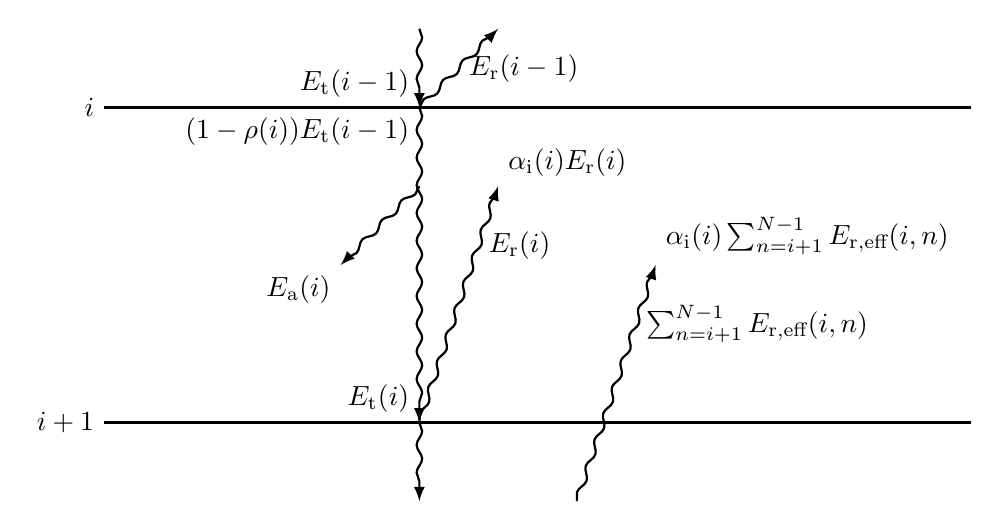
\begin{tikzpicture}[
  thick,
  radiation/.style={
    -latex,
    decorate,
    decoration={
      snake,
      amplitude=1,
      post length=1mm
    }
  }
]
  \draw[radiation] (0,1) -- (0,0)
    node[anchor=south east] {$E_\text{t}(i - 1)$};
  \draw[radiation] (0,0) -- (1,1)
    node[midway,anchor=west] {$E_\text{r}(i - 1)$};
  \draw (-4,0)
    node[anchor=east] {$i$}
    -- (7,0);
  \draw[radiation] (0,0)
    node[anchor=north east] {$(1 - \rho(i)) E_\text{t}(i - 1)$}
    -- (0,-4)
    node[anchor=south east] {$E_\text{t}(i)$};
  \draw[radiation] (0,-1) -- (-1,-2)
    node[anchor=north east] {$E_\text{a}(i)$};
  \draw[radiation] (0,-4) -- (1,-1)
    node[anchor=south west] {$\alpha_\text{i}(i) E_\text{r}(i)$}
    node[near end,anchor=west] {$E_\text{r}(i)$};
  \draw (-4,-4)
    node[anchor=east] {$i + 1$}
    -- (7,-4);
  \draw[radiation] (0,-4) -- (0,-5);
  \draw[radiation] (2,-5) -- (3,-2)
    node[anchor=south west] {$\alpha_\text{i}(i) \sum_{n = i + 1}^{N - 1} E_{\text{r},\text{eff}}(i, n)$}
    node[near end,anchor=west] {$\sum_{n = i + 1}^{N - 1} E_{\text{r},\text{eff}}(i, n)$};
\end{tikzpicture}
\end{document}
